In this section, we evaluate two fundamental problems inherent to the weighted-average interpolation method: 1) comb-filtering introduced by summing two very similar signals separated by a time delay and 2) localization errors due to the precedence effect.
In the following analyses, we consider a sound field consisting of a two-microphone array and a single point-source, as described in \secref{sec:06_Simulation_Framework:Linear_Geometry} and illustrated in \figref{fig:06_Simulation_Framework:Linear_Geometry}.

%%%% Comb-filtering %%%%
\subsection{Coloration: comb-filtering}
For a plane-wave source (i.e., $s_0 \to \infty$),
the path-length difference from the source to each microphone is $\Delta \sin |\varphi_0|$,
and the corresponding time-of-arrival delay is $(\Delta / c) \sin |\varphi_0|$, where $c$ is the speed of sound.
For a listener at the origin, the interpolation weights are given by $w_1 = w_2 = 0.5$.\footnote{More generally, $w_1 = 0.5 + y_0/\Delta$ and $w_2 = 0.5 - y_0/\Delta$ for $y_0 \in [-\Delta/2,\Delta/2]$.}
Thus the weighted-average impulse response for the zeroth-order (i.e., omnidirectional) ambisonics signal\footnote{Note that the subscript of $a_n$ refers to the ambisonics channel number (ACN), as described in \secref{sec:02_Acoustical_Theory:Definitions}.} is given by
\begin{equation}
a_0(t) = 0.5 \delta(t) + 0.5 \delta \left(t - \frac{\Delta}{c} \sin \left|\varphi_0\right| \right),
\end{equation}
where $\delta(t)$ is the Dirac delta function, and the corresponding frequency response is given by
\begin{equation}
A_0(k) = 0.5 + 0.5 e^{-i k \Delta \sin \left|\varphi_0\right|},
\end{equation}
where $k = 2 \pi f / c$ is the angular wavenumber for frequency $f$.
As this frequency response depends only on $|\varphi_0|$ and the nondimensional frequency $k\Delta$,
we plot, in~\figref{fig:08_Proposed_Method:XF_CombFiltering_NonDim}, magnitude responses of $A_0$ as a function of the nondimensional wavenumber $k\Delta \sin|\varphi_0|$.
Note that the lowest-frequency notch occurs at $k\Delta \sin|\varphi_0| = \pi$; more generally, notches occur at all $k\Delta \sin|\varphi_0| = (2n-1)\pi,~\forall n = 1,2,3,\dots$.

% Comb-filter magnitude responses
\begin{figure}[t]
\centering
  \includegraphics[width = 0.49\textwidth]{08_proposed_method/figures/nonDimFreqResp_xf.eps}
  \caption{Comb-filter magnitude responses caused by the weighted average method.}
  \label{fig:08_Proposed_Method:XF_CombFiltering_NonDim}
\end{figure} %%NOTE%% vertical axis label is too complicated: |A0 / B0ref| or something

Similarly, in \figref{fig:08_Proposed_Method:XF_CombFiltering}, we plot the same magnitude responses of $A_0$ but for a fixed microphone spacing of $\Delta = 0.5$~m and for particular source azimuths.
Note that due to the lateral symmetry of the geometry, these responses hold for negative azimuths ($\varphi_0' = -\varphi_0$),
and due to the front-back symmetry, they also hold for rear azimuths ($\varphi_0' = 180^\circ \pm \varphi_0$).
From this plot, we see that only sources at $0^\circ$ (or $180^\circ$) azimuth are interpolated without comb-filtering.
For all other azimuths, comb-filtering is introduced due to the time-of-arrival delay between microphones.

\begin{figure}[t]
\centering
  \includegraphics[width = 0.49\textwidth]{08_proposed_method/figures/freqResp_xf.eps}
  \caption[Comb-filter magnitude responses caused by the weighted average method.]{
  Comb-filter magnitude responses caused by the weighted average method for various source azimuths.
  The bottom axis shows frequency in kHz for a microphone spacing of $\Delta = 0.5$~m while the top axis shows the nondimensional frequency $k\Delta$.
  For legibility, each frequency response is offset by $50$~dB and notch depths have been artificially truncated to not exceed $-45$~dB.}
  \label{fig:08_Proposed_Method:XF_CombFiltering}
\end{figure} %%NOTE%% vertical axis label is too complicated: |A0 / B0ref| or something

%%%% Precedence-effect errors %%%%
\subsection{Localization: precedence-effect errors}
For a plane-wave source, the localization information received by each microphone will be identical, so localization of the interpolated signal is likely unchanged.
However, for a finite-distance source, the apparent source direction will differ between the perspectives of each microphone.
In such cases, interpolation between the microphones effectively leads to the creation of distinct \textit{virtual sources}, as illustrated in~\figref{fig:08_Proposed_Method:Effective_Sources}.

% Diagram of effective source positions
\begin{figure}[t]
\centering
  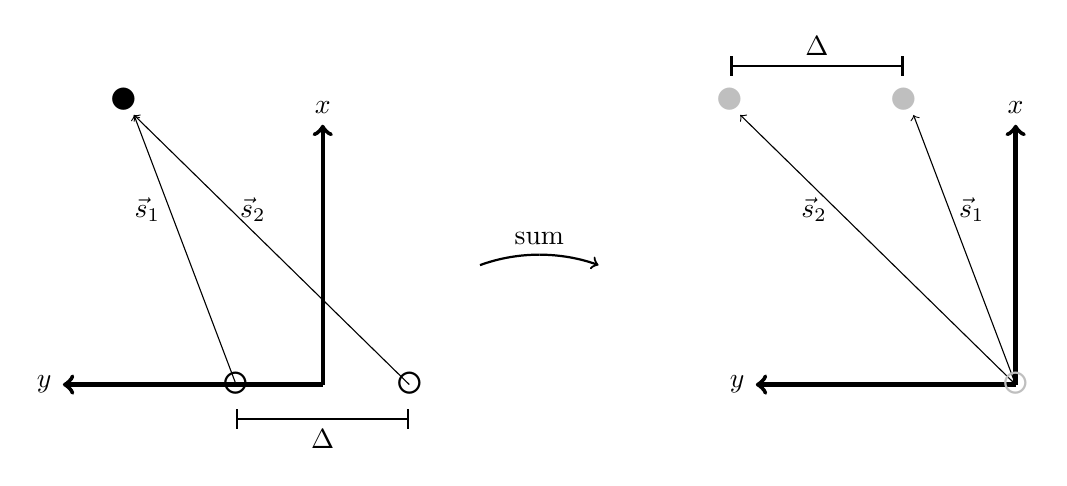
\begin{tikzpicture}[scale=2.2]
% Parameters
\def\radius{1.5};
\def\arrowScale{0.95};
\def\plotOffset{2}

\def\micSpacing{1};
\def\micL{-0.5*\micSpacing};
\def\micR{0.5*\micSpacing};

\def\sourceRadius{2};
\def\sourceAzimuth{35}
\pgfmathsetmacro\sourceY{cos(-\sourceAzimuth)*\sourceRadius}
\pgfmathsetmacro\sourceX{sin(-\sourceAzimuth)*\sourceRadius}

\pgfmathsetmacro\sourceLAzimuth{-atan((\sourceX-\micL)/\sourceY)}
\pgfmathsetmacro\sourceRAzimuth{-atan((\sourceX-\micR)/\sourceY)}

% Coordinate system
\draw[ultra thick,->] (0-\plotOffset,0) -- (0-\plotOffset,\radius) node[above]{$x$};
\draw[ultra thick,->] (0-\plotOffset,0) -- (-\radius-\plotOffset,0) node[left]{$y$};

% Source
\node at (\sourceX-\plotOffset,\sourceY){\huge $\bullet$}; % source
\draw[->] (\micL-\plotOffset,0) -- (\arrowScale*\sourceX-\plotOffset,\arrowScale*\sourceY) node[left, pos=0.65]{$\vec{s}_1$}; % left mic
\draw[->] (\micR-\plotOffset,0) -- (\arrowScale*\sourceX-\plotOffset,\arrowScale*\sourceY) node[right, pos=0.65]{$\vec{s}_2$}; % right mic

% Mic positions
\node at (\micL-\plotOffset,0){\huge $\circ$};
\node at (\micR-\plotOffset,0){\huge $\circ$};
\draw[thick,|-|] (\micL-\plotOffset,-0.2) -- (\micR-\plotOffset,-0.2) node[below, pos=0.5]{$\Delta$};

% Transformation
\draw[thick,-] (0-\radius/2,\radius/2) arc(90:110:1cm); \draw[thick,->] (0-\radius/2,\radius/2) node[above]{sum} arc(90:70:1cm);

% Effective coordinate system
\draw[ultra thick,->] (0+\plotOffset,0) -- (0+\plotOffset,\radius) node[above]{$x$};
\draw[ultra thick,->] (0+\plotOffset,0) -- (-\radius+\plotOffset,0) node[left]{$y$};

% Effective sources
\node at (\sourceX+\plotOffset+\micL,\sourceY){\huge $\color{lightgray}{\bullet}$}; % left source
\node at (\sourceX+\plotOffset+\micR,\sourceY){\huge $\color{lightgray}{\bullet}$}; % right source
\draw[->] (0+\plotOffset,0) -- (\arrowScale*\sourceX+\plotOffset-\micL,\arrowScale*\sourceY) node[right, pos=0.65]{$\vec{s}_1$}; % left mic
\draw[->] (0+\plotOffset,0) -- (\arrowScale*\sourceX+\plotOffset-\micR,\arrowScale*\sourceY) node[left, pos=0.65]{$\vec{s}_2$}; % right mic

% Effective mic position
\node at (0+\plotOffset,0){\huge $\color{lightgray}{\circ}$};
\draw[thick,|-|] (\micL+\plotOffset+\sourceX,\sourceY+0.2) -- (\micR+\plotOffset+\sourceX,\sourceY+0.2) node[above, pos=0.5]{$\Delta$};

\end{tikzpicture}
  \caption[Diagram of virtual sources created by the weighted average method.]{
  Diagram of virtual sources (light gray filled circles) effectively created by the weighted average method for a pair of microphones (empty circles) in a sound field with a single source (black filled circle).}
  \label{fig:08_Proposed_Method:Effective_Sources}
\end{figure}

To explore the potential localization errors created by these virtual sources, we employ the precedence-effect-based localization model of \citet{Stitt2016}, as described here in \secref{sec:04_Auditory_Models:PE_Energy_Vector}.
This model takes as inputs the source positions (in this case, $\vec{s}_1$ and $\vec{s}_2$) and signal amplitudes (the interpolation weights $w_1$ and $w_2$ from \eqnref{eq:03_Navigation_Techniques:Crossfading}), and computes a predicted localization vector, $\vec{\nu}_\text{PE}$.
Here we let the free parameter, $\alpha$, as defined by~\citeauthor{Stitt2016}, take a value of $\alpha = 0.6$, which is somewhat typical for a stimulus signal consisting of both transient and stationary components \citep{Stitt2016}.
We then compute, using the real source position ($\vec{s}_0$) and the desired listener position ($\vec{r}_0$), a localization error, $e_\nu$, given by \eqnref{eq:04_Auditory_Models:Localization_Error} with $\vec{\nu}$ replaced by $\vec{\nu}_\text{PE}$ (and with $\vec{s}_0{}' = \vec{s}_0 - \vec{r}_0$).
%\begin{equation}\label{eq:08_Proposed_Method:Localization_Error}
%e_\nu = \cos^{-1} \left( \hat{\nu}_\text{PE} \cdot \frac{\vec{s}_0 - \vec{r}_0}{\|\vec{s}_0 - \vec{r}_0\|} \right),
%\end{equation}
%where $\|\cdot\|$ denotes the $\ell^2$ norm (Euclidean distance) of a vector.

In \figref{fig:08_Proposed_Method:XF_PrecedenceErrors}, we plot these predicted localization errors, averaged over the entire navigable region (as defined in \secref{sec:06_Simulation_Framework:Linear_Geometry}) and all source azimuths, for various combinations of source distance $s_0$ and microphone spacing $\Delta$.
%In this simulation, we vary the source azimuth from $\varphi_0 = 0^\circ$ to $90^\circ$ in increments of $5^\circ$, and the listener position from $y_0 = -\Delta/2$ to $\Delta/2$ in 30 equal increments.
Note that we exclude from this contour plot the region in which $s_0 + \Delta / 2 < 0.1$~m
(i.e., the bottom left corner of \figref{fig:08_Proposed_Method:XF_PrecedenceErrors}), as this corresponds to geometries for which the source is
``inside the head'' (for an approximate head radius of 10~cm) at all positions within the navigable region.

\begin{figure}[t]
\centering
  \includegraphics[width = 0.49\textwidth]{08_proposed_method/figures/stitt2016_a60_contour_xf.eps}
  \caption[Localization contour plot for the weighted average method.]{
  Predicted localization errors $e_\nu$ incurred by the weighted average method
  for various combinations of microphone spacing $\Delta$ and normalized source distance $\gamma = s_0 / (\Delta / 2)$.
  The plotted errors have been averaged over the entire navigable region (as defined in~\secref{sec:06_Simulation_Framework:Linear_Geometry})
  and all source azimuths ($\varphi_0 \in [0,90^\circ]$ in increments of $5^\circ$).
  Contour lines are drawn every $5^\circ$.}
  \label{fig:08_Proposed_Method:XF_PrecedenceErrors}
\end{figure}

From this plot, we first note that localization errors appear primarily dependent on $\gamma$, but tend to increase with increasing $\Delta$.
We also see that, at large microphone spacings ($\Delta > 0.5$~m), localization errors for ``slightly'' interior sources ($0.5 < \gamma < 1$) become extreme ($e_\nu > 50^\circ$).
Localization errors for distant exterior sources ($\gamma > 2$), however, are uniformly small ($e_\nu < 10^\circ$).
Although not shown here, it can be verified that these localization errors tend to decrease with increasing $\alpha \in [0,1]$,
as $\alpha = 1$ corresponds to purely energy-based localization, with no effect from time-of-arrival delays \citep{Stitt2016}.
Consequently, as $\alpha \to 1$, the dependence of $e_\nu$ on $\Delta$ disappears.